\documentclass[../xlapes02]{subfiles}
\begin{document}
    \chapter{Experiments and Results}\label{ch:experiments-and-results}
    In this chapter, we will present the outcomes of our experiments, including any issues encountered during the experimentation process.\ We demonstrate the performance of our agent in a given environment through a series of experiments and provide additional details on hyperparameter selection and comparison of different hyperparameter settings in~\cref{sec:first-experiment:-hyperparameter-tuning}.\ We also evaluate and compare the advantages and disadvantages of the datasets used in training our model in~\ref{sec:datasets-impact}, with a focus on identifying the most appropriate dataset.\ The robustness of our model is assessed in~\ref{sec:testing-of-robustness}.\ Furthermore, we compare the performance of our model with standard indices such as the \emph{S\&P 500 Index} and \emph{DJI Index}, and discuss the results of our experiments with baseline models and benchmarks.\ To maintain consistency in our results, we primarily compare our model's performance with the DJI Index as the datasets are derived from companies in the DJI Index.\ However, we also compare our results with other indices and \emph{State-of-the-Art AI4Finance} in~\ref{sec:baselines-and-backtesting}.\ All experiments were documented during our testing period from \textbf{2017-01-25} to \textbf{2022-12-16}.\ Last assessment will involve examining important portfolio metrics, as described in~\cref{sec:portfolio-metrics-comparison}.\ Finally, we summarize our findings and discuss the results of our experiments in~\ref{sec:summary}.

    In addition, we provide details of our approach to performance testing and the MLOps concepts used, including tracking training and testing of our models, in Section~\ref{subsec:wandb}.

%    \paragraph{Reproducibility}\label{par:reproducibility}
    To ensure \emph{Reproducibility} of our work we also make publicly available on the W\&B website all datasets, models, and training/testing logs with a history of all hyperparameters for each algorithm. \textbf{By visiting the following URL: \url{https://wandb.ai/investai/portfolio-allocation}}, anyone can access the results of each run, and reproduce our findings while comparing them with their own experiments.


    \section{Hardware \& Tools}\label{sec:hardware-tools}

    \subsection{Hardware}\label{subsec:hardware}
    The computer used for experiments has the following specifications:
    \begin{itemize}
        \item Operating System: Ubuntu 20.04.6 LTS (GNU/Linux 5.4.0-146-generic x86\_64)
        \item CPU: 2 x Intel Xeon CPU E5-2620 v3 @ 2.40GHz, each with six cores, for a total of 12 cores.
        \item RAM: 2 x 32 GB RAM running at 2133MHz, using quad-channel architecture for faster memory access
        \item GPU: 4 x NVIDIA GTX 1080 (Pascal) with 8GB RAM each, providing a total of 32GB GPU memory.
    \end{itemize}

    \subsection{Weights \& Biases}\label{subsec:wandb}
    Weights \& Biases (W\&B) is a powerful ML experiment tracking and visualization tool that helps data scientists and machine learning practitioners manage their experiments.\ With W\&B, users can log experiment metrics in real-time, track hyperparameters, and compare and reproduce experiments easily.\ W\&B offers various visualization tools like interactive plots, histograms, and confusion matrices, which help users analyze and understand experimental results.

    \begin{itemize}
        \item Experiment tracking: W\&B allows users to log experiment metrics such as loss, accuracy, and other custom metrics in real-time during training.\ These metrics are logged to a central dashboard, making it easy to monitor and compare multiple experiments.
        \item Hyperparameter tuning: W\&B supports hyperparameter sweeps, allowing users to explore different hyperparameter configurations in parallel and find optimal hyperparameter settings for their models.
        \item Visualization: W\&B provides a variety of visualization tools, including interactive graphs, histograms, confusion matrices, and more, to help users analyze and understand experimental results.\ We use some of the W\&B graphs to compare hyperparameters and their values to understand their effect on the overall range of rewards~\cref{sec:hyperparameters-tuning-results}.
        \item Artifact management: W\&B allows users to log and version datasets, models, and other artifacts, making it easy to track and reproduce experiments with specific data and model versions.
        \item Collaboration: W\&B enables team collaboration by allowing users to share experiment results, visualizations, and artifacts with team members, facilitating communication and collaboration among team members.
    \end{itemize}

    Due to the variety of features available through the W\&B API, we have chosen not to provide a comprehensive description of each one.\ However, we recommend looking at the W\&B documentation available at \url{https://docs.wandb.ai/} for an explanation of all APIs and features.


    \section{Focus of the experiments}\label{sec:focus-of-the-experiments}
    Our aim is to determine the best \emph{hyperparameters} and \emph{datasets} for training and testing, that provide the agent to get the highest portfolio value over time.\ To achieve this, we use a \emph{hyperparameter sweeping} approach to testing the hyperparameters for each algorithm and dataset.\ The performance of each hyperparameter configuration is determined based on the model's output, using a metric named as \emph{test/total\_reward}.\ This metric represents the cumulative product of the portfolio value, as described by the equation in~\cref{eq:portfolio-value} and then further described in~\cref{subsec:how_we_calculate_agent_performance}.\ The higher the value of \emph{test/total\_reward}, the better the performance of the model.

    We compare the best and worst performing models with State-of-the-Art AI4Finance and common indexes and strategies as baselines.\ Our results indicate that appropriate hyperparameters and good featured datasets can train the agent sufficiently well to outperform common indexes and other publicly available models for Portfolio Allocation (using Reinforcement Learning).\ This makes them valuable tools for portfolio allocation in financial markets.

    Thus, the main goal of this chapter is to evaluate the trained models' performance through rigorous experimentation and identify the best \emph{hyperparameters} and \emph{datasets} for optimal performance.\

    We also test the model's \emph{robustness} by assessing its stability using the best hyperparameters for the dataset and the specific algorithm used to train the model.\ This helps us ensure that the model is reliable and can perform consistently well under different conditions.\ The robustness test helps us identify potential weaknesses or limitations that may need to be addressed.


    \section{First experiment: Hyperparameter Tuning}\label{sec:first-experiment:-hyperparameter-tuning}
    Since the configuration of hyperparameters is crucial for the performance of any machine-learning model.\ We performed a hyperparameter sweep to find the best hyperparameters for our models through a bunch of hyperparameters shown in~\cref{tab:hyperparameters}.\ In this case, the hyperparameter sweep was performed on 27 hyperparameters using the Weights \& Biases Sweep, this helps us to track and visualize the training process and store a bunch of hyperparameter configurations.\ The range or value of each hyperparameter was chosen based on prior knowledge.

    \subsection{Time Steps}\label{subsec:time_steps}
    The only hyperparameter, which stays the same throughout \emph{hyperparameter sweeping} was \emph{Time Steps} parameter.\ We conducted experiments by varying its value from $20000$ to $100000$ and found that values up to $50,000$ still improve the model's performance.\ However, values above $50000$ did not provide any significant improvement in the model's performance, and the training time increased considerably.\ As a result, we decided to use \textbf{50000 time steps} for all the models that we experimented with in this chapter.

    \subsection{Selection of hyperparameters}\label{subsec:selection_of_hyperparameters}
    In this subsection, we will discuss other hyperparameters and explain how we selected the range of values for them.\ Once the range or values of each hyperparameter was set, as shown in~\cref{tab:hyperparameters}, the process of finding the best configuration of hyperparameters was a kind of brute force, except that we at least restrict the exploration space in which the W\&B Sweep is trying to find optimal hyperparameter through randomly selecting each hyperparameter for the given run.

    The Sweep involved \textbf{5 distinct} reinforcement learning algorithms - namely \emph{A2C}, \emph{PPO}, \emph{SAC}, \emph{DDPG}, and \emph{TD3} - and each of these algorithms was trained on \textbf{3 unique datasets}, which were introduced in the preceding chapter and referred to as Fundamental, Technical, and Combined.\ In total, this resulted in \textbf{15 different combinations} of algorithms and datasets.\ Furthermore, each combination was subjected to \textbf{10 rounds} of training, culminating in a total of \textbf{150 train/test runs}.\ These runs are accessible on W\&B at the following URL: \url{https://wandb.ai/investai/portfolio-allocation}.

    It is worth emphasizing that when performing a hyperparameter sweep, certain hyperparameters may be selected even though the algorithm does not require them, that means in such cases, we simply \emph{discard} those unnecessary chosen hyperparameters and only pass the necessary ones to the algorithm.

    In~\cref{tab:hyperparameters}, the hyperparameters that underwent tuning during the hyperparameter sweep are displayed.\ The values enclosed in $<>$ indicate the range from which W\&B Sweep can randomly select a value for a particular run, while those enclosed in $[\ ]$ represent the list of values from which W\&B Sweep can randomly choose a value for a particular run.\ The performance of the agent with respect to the hyperparameters is presented in the graphs, which compare and analyze the performance of several of the best and worst models.\ These graphs can be found in~\cref{sec:hyperparameters-tuning-results}.

    \begin{table}[H]
        \centering
        {\footnotesize
            \begin{tabular}{|l|c|}
                \hline
                \textbf{Parameter}        & \textbf{Values/range}                           \\ \hline
                learning\_rate            & <0.0001, 0.01>                                  \\ \hline
                n\_steps                  & [32, 64, 128, 256, 512, 1024, 2048]             \\ \hline
                gamma                     & <0.9, 0.999>                                    \\ \hline
                gae\_lambda               & <0.8, 0.999>                                    \\ \hline
                ent\_coef                 & <0.0001, 0.01>                                  \\ \hline
                vf\_coef                  & <0.0001, 0.01>                                  \\ \hline
                max\_grad\_norm           & <0.5, 0.99>                                     \\ \hline
                rms\_prop\_eps            & <0.0001, 0.01>                                  \\ \hline
                sde\_sample\_freq         & <4, 32>                                         \\ \hline
                batch\_size               & [32, 64, 128, 256, 512, 1024, 2048, 4096, 8192] \\ \hline
                n\_epochs                 & <1, 10>                                         \\ \hline
                clip\_range               & <0.1, 0.3>                                      \\ \hline
                clip\_range\_vf           & [None, 0.05, 0.1, 0.15, 0.2]                    \\ \hline
                target\_kl                & <0.01, 0.05>                                    \\ \hline
                buffer\_size              & [1000, 2000, 3000, 4000, 5000]                  \\ \hline
                learning\_starts          & <100, 1000>                                     \\ \hline
                tau                       & <0.001, 0.01>                                   \\ \hline
                train\_freq               & <1, 4>                                          \\ \hline
                gradient\_steps           & <1, 4>                                          \\ \hline
                target\_update\_interval  & <1, 4>                                          \\ \hline
                target\_entropy           & <0.1, 0.2>                                      \\ \hline
                policy\_delay             & <1, 4>                                          \\ \hline
                target\_policy\_noise     & <0.1, 0.2>                                      \\ \hline
                target\_noise\_clip       & <0.1, 0.2>                                      \\ \hline
                exploration\_fraction     & <0.1, 0.2>                                      \\ \hline
                exploration\_initial\_eps & <0.1, 0.2>                                      \\ \hline
                exploration\_final\_eps   & <0.1, 0.2>                                      \\ \hline
            \end{tabular}
        }
        \caption{Hyperparameters range/values to select from, for the hyperparameter sweep.}
        \label{tab:hyperparameters}
    \end{table}

    \subsection{Hyperparameter Sweep Results}\label{subsec:hyperparameter_sweep_results}
    We evaluate the agent's performance based on \emph{test/total\_reward} attribute.\ In~\cref{sec:hyperparameters-tuning-results} is shown how the hyperparameter tuning was performed on given hyperparameters and how much each influenced the \emph{test/total\_reward}.\ It distinguishes individual training runs, and the color of the curve corresponds to its value, a higher value of \emph{test/total\_reward} is represented by an \textcolor[RGB]{255,128,0}{orange curve, indicating better performance}, conversely, a lower value is represented by a \textcolor[RGB]{100,0,200}{purple curve, indicating poor performance}.\ These graphs have two columns: the first column represents the \emph{algorithm}, and the last column represents the \emph{test/total\_reward}.\ The hyperparameters, which were tuned during the hyperparameter sweep, are located between these two columns.\ Including three graphs instead of one makes the results more readable and easier to analyze.

    The~\cref{tab:best-worst-hyperparameters} presents the configurations of the top 2 and bottom 2 models, including their hyperparameters and the corresponding \emph{test/total\_reward} values.

    \begin{table}[H]
        \centering
        {\footnotesize
            \begin{tabular}{|l||l|l||l|l|}
                \hline
                \textbf{Model ID}                  & p3irnh80                                     & 8tml2ozg                                     & zfjr0ks0                                     & pky1wslb                                     \\ \hline
                \textbf{algo}                      & DDPG                                         & A2C                                          & A2C                                          & PPO                                          \\ \hline
                \textbf{learning\_rate}            & 0.00685                                      & 0.00671                                      & 0.00698                                      & 0.00471                                      \\ \hline
                \textbf{n\_steps}                  & 256                                          & 128                                          & 128                                          & 32                                           \\ \hline
                \textbf{gamma}                     & 0.9294                                       & 0.94108                                      & 0.93858                                      & 0.9289                                       \\ \hline
                \textbf{gae\_lambda}               & 0.99624                                      & 0.90203                                      & 0.9383                                       & 0.85115                                      \\ \hline
                \textbf{ent\_coef}                 & 0.00203                                      & 0.0013                                       & 0.00525                                      & 0.00173                                      \\ \hline
                \textbf{vf\_coef}                  & 0.0082                                       & 0.00683                                      & 0.00125                                      & 0.00527                                      \\ \hline
                \textbf{max\_grad\_norm}           & 0.71475                                      & 0.56558                                      & 0.94281                                      & 0.77201                                      \\ \hline
                \textbf{rms\_prop\_eps}            & 0.00024                                      & 0.00435                                      & 0.0075                                       & 0.0067                                       \\ \hline
                \textbf{sde\_sample\_freq}         & 30                                           & 26                                           & 23                                           & 15                                           \\ \hline
                \textbf{batch\_size}               & 128                                          & 64                                           & 8192                                         & 64                                           \\ \hline
                \textbf{n\_epochs}                 & 5                                            & 8                                            & 7                                            & 8                                            \\ \hline
                \textbf{clip\_range}               & 0.18938                                      & 0.19559                                      & 0.2274                                       & 0.22578                                      \\ \hline
                \textbf{clip\_range\_vf}           & 0.05                                         & ~                                            & 0.15                                         & 0.05                                         \\ \hline
                \textbf{target\_kl}                & 0.02394                                      & 0.04957                                      & 0.03176                                      & 0.03337                                      \\ \hline
                \textbf{buffer\_size}              & 2000                                         & 5000                                         & 2000                                         & 2000                                         \\ \hline
                \textbf{learning\_starts}          & 387                                          & 163                                          & 569                                          & 165                                          \\ \hline
                \textbf{tau}                       & 0.00815                                      & 0.00461                                      & 0.00269                                      & 0.00469                                      \\ \hline
                \textbf{train\_freq}               & 2                                            & 2                                            & 3                                            & 2                                            \\ \hline
                \textbf{gradient\_steps}           & 1                                            & 3                                            & 1                                            & 3                                            \\ \hline
                \textbf{target\_update\_interval}  & 3                                            & 2                                            & 4                                            & 2                                            \\ \hline
                \textbf{target\_entropy}           & 0.19013                                      & 0.15826                                      & 0.18233                                      & 0.13979                                      \\ \hline
                \textbf{policy\_delay}             & 2                                            & 4                                            & 2                                            & 3                                            \\ \hline
                \textbf{target\_policy\_noise}     & 0.11459                                      & 0.15052                                      & 0.10674                                      & 0.12649                                      \\ \hline
                \textbf{target\_noise\_clip}       & 0.18538                                      & 0.10527                                      & 0.18672                                      & 0.14197                                      \\ \hline
                \textbf{exploration\_fraction}     & 0.12082                                      & 0.10871                                      & 0.16125                                      & 0.16269                                      \\ \hline
                \textbf{exploration\_final\_eps}   & 0.18574                                      & 0.10366                                      & 0.10618                                      & 0.19131                                      \\ \hline
                \textbf{exploration\_initial\_eps} & 0.16609                                      & 0.10003                                      & 0.16434                                      & 0.1039                                       \\ \hline
                \textbf{test/total\_reward}        & \textcolor[RGB]{50,150,50}{\textbf{1.97214}} & \textcolor[RGB]{50,150,50}{\textbf{1.97061}} & \textcolor[RGB]{150,50,50}{\textbf{1.62093}} & \textcolor[RGB]{150,50,50}{\textbf{1.63348}} \\ \hline
            \end{tabular}
        }
        \caption{Best and worst model and their training hyperparameters. All hyperparameters are also available online URL: \url{https://wandb.ai/investai/portfolio-allocation} with much more details and experiments.}
        \label{tab:best-worst-hyperparameters}
    \end{table}


    \section{Datasets Impact}\label{sec:datasets-impact}
    In this section, we will assess the models based on the \emph{datasets} they were trained on.\ Specifically, we will show and evaluate the \textbf{6 best} and \textbf{6 worst} agents/models according to the specific datasets (\emph{Fundamental}, \emph{Technical}, and \emph{Combined}).\ The outcomes of this comparison are presented in~\cref{tab:datasets-comparison}.\ Although the results in~\cref{tab:datasets-comparison} may vary depending on the hyperparameters, we can still observe that the \emph{Technical Dataset} is the worst, while the \emph{Combined Dataset} is the best, and the \emph{Fundamental Dataset} is good enough for training the agent.

    Our assumption that the \textbf{Fundamental Dataset} would be sufficient for training a profitable agent has been confirmed, although the \textbf{Combined Dataset} can yield better results despite being more complex and difficult to train.\ As expected, the \textbf{Technical Dataset} performed the worst, as technical indicators are not as reliable as fundamental indicators for assessing the health and future growth of a company.\ Since the \emph{Technical Analysis} is based on the assumption that the past price movements can predict future price movements, it is not surprising that the \emph{Technical Dataset} performed the worst and it shows that the market history does not guarantee the same results in the future.

    \begin{table}[H]
        \centering
        \begin{tabular}{|l|l|l|}
            \hline
            \textbf{Model ID} & \textbf{Dataset Type} & \textbf{test/total\_reward}                \\ \hline
            p3irnh80          & Combined              & \textcolor[RGB]{50,150,50}{\textbf{1.972}} \\ \hline
            8tml2ozg          & Combined              & \textcolor[RGB]{50,150,50}{\textbf{1.970}} \\ \hline
            geaioz9h          & Fundamental           & \textcolor[RGB]{50,150,50}{\textbf{1.965}} \\ \hline
            8iq9e37s          & Combined              & \textcolor[RGB]{50,150,50}{\textbf{1.956}} \\ \hline
            y3zz2sv3          & Combined              & \textcolor[RGB]{50,150,50}{\textbf{1.955}} \\ \hline
            4qr3nk43          & Fundamental           & \textcolor[RGB]{50,150,50}{\textbf{1.945}} \\
            \midrule
            \midrule
            zfjr0ks0          & Fundamental           & \textcolor[RGB]{150,50,50}{\textbf{1.620}} \\ \hline
            pky1wslb          & Combined              & \textcolor[RGB]{150,50,50}{\textbf{1.633}} \\ \hline
            2161deh4          & Technical             & \textcolor[RGB]{150,50,50}{\textbf{1.642}} \\ \hline
            ipl1v8io          & Technical             & \textcolor[RGB]{150,50,50}{\textbf{1.643}} \\ \hline
            2161deh4          & Technical             & \textcolor[RGB]{150,50,50}{\textbf{1.642}} \\ \hline
            2161deh4          & Technical             & \textcolor[RGB]{150,50,50}{\textbf{1.642}} \\ \hline
        \end{tabular}
        \caption{Examples of 6 best models in the upper part and 6 worst models in the lower part of the table.}
        \label{tab:datasets-comparison}
    \end{table}


    \section{Testing of Robustness}\label{sec:testing-of-robustness}
    In this section, we will examine whether the hyperparameters setup, which seems the best (\emph{p3irnh80}) is robust or not by conducting multiple tests on the models and training them with the same hyperparameters.\ We trained \textbf{11 models} using the same hyperparameters but different \emph{seeds}, and tested them all on the \emph{Combined Dataset}.\ The results are summarized in~\cref{tab:robust}, which shows the \emph{test/total\_reward} for each of the 11 models.\ The mean \emph{test/total\_reward} across the models is \textbf{1.824}, indicating that the models perform well on the test dataset.\ Although there is some variation in performance between the models, with a spread of \textbf{0.249} between the highest and lowest cumulative reward values (\emph{test/total\_reward}), the distinction is significant since it has the potential to greatly impact the long-term returns.\ Overall, these results suggest that the models are robust enough to be used in real-life scenarios.\ It is worth noting that the variation in performance between the models may be due to differences in the random seeds used during training, which can affect the initial conditions of the learning process.

    \begin{table}[H]
        \centering
        \caption{Robust Test: Trained models using hyperparameters from the best model trained using sweep. The mean is 1.824 and the spread between the highest and the lowest reward is 0.249.}
        \label{tab:robust}
        {\footnotesize\begin{tabular}{*{2}{|m{0.20\linewidth}|}}
                          \toprule
                          \bfseries Model ID & \bfseries test/total\_reward \\[0cm]
                          \midrule
                          \bfseries kyr89ols & 1.723 \\[0cm]
                          \bfseries l75jybwn & 1.769 \\[0cm]
                          \bfseries axq1epdr & 1.776 \\[0cm]
                          \bfseries 3hiqutvc & 1.785 \\[0cm]
                          \bfseries sey6enti & 1.799 \\[0cm]
                          \bfseries w1xo3vul & 1.806 \\[0cm]
                          \bfseries 4y7nkqyj & 1.807 \\[0cm]
                          \bfseries mliee6kz & 1.864 \\[0cm]
                          \bfseries e5pzquaz & 1.882 \\[0cm]
                          \bfseries r92of0f3 & 1.887 \\[0cm]
                          \bfseries p3irnh80 & 1.972 \\[0cm]
                          \bottomrule
        \end{tabular}}
    \end{table}


    \section{Baselines \& Benchmarks}\label{sec:baselines-and-backtesting}
    In this section, we compare the performance of the agent to several baselines, including well-known market indexes as: \textbf{The S\&P 500 Index (GSPC)},\textbf{The Dow Jones Industrial Average (DJI)}, \textbf{The Russell 2000 (RUT)}, \textbf{The NASDAQ Composite (IXIC)}. And in our comparison, we also incorporate investment strategies as \textbf{Minimum Variance}, \textbf{Maximum Sharpe Ratio}~\cite{investopedia}.

    \subsection{Comparing Portfolio Performance: Analysis from 2017 to 2022}\label{subsec:cumulative-returns}
    In~\cref{fig:cumulative_return}, we demonstrate that an agent can achieve successful outcomes when trained with appropriate hyperparameters and dataset (model id: \emph{zfjr0ks0}), while unsuitable hyperparameters and dataset can result in unsatisfactory outcomes (model id: \emph{p3irnh80}). The \emph{zfjr0ks0} model surpassed standard indexes such as \emph{DJI}, \emph{GSPC}, \emph{IXIC}, and \emph{RUT}, although not consistently throughout the testing period.\ It is evident that the \emph{zfjr0ks0} model outperformed almost all baseline indexes and strategies, with the exception of \emph{IXIC (NASDAQ Composite)} during a specific period from 2020 until the end of the testing period in 2022, when our model began to outperform even \emph{IXIC}. There could be various reasons why our agent was outperformed by the Nasdaq 100 during the testing period.\ However, we believe that the primary reason is that our \emph{agent} is designed to operate with only \textbf{30 stocks}, while the \emph{NASDAQ Comosite} comprises \textbf{100 stocks}.\ This limited scope of stocks may have resulted in fewer investment opportunities for our agent, which could have led to lower returns compared to the Nasdaq 100.\ Nonetheless, it is worth noting that our model did eventually outperform the Nasdaq 100 Index by the end of 2023.

    Currently, we lack adequate data to conduct a thorough comparison between our developed model and the State-of-the-Art AI4Finance.\ However, in the following subsection where we will have the necessary data, we intend to perform a comprehensive comparison.
    \begin{figure}
        \centering
        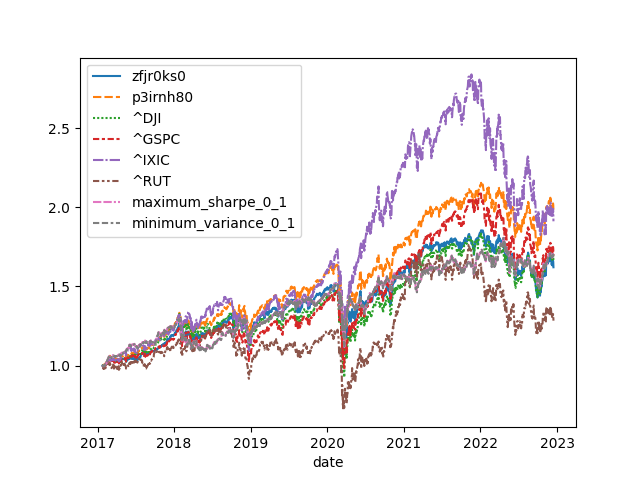
\includegraphics[width=0.85\linewidth]{image/figure/returns}
        \caption{Cumulative returns of the best(zfjr0ks0) and worst(p3irnh80) performing models, indexes (DJI, GSPC, IXIC, RUT), and strategies (minimum variance and maximum Sharpe ratio), during the testing period (2017-2022).}
        \label{fig:cumulative_return}
    \end{figure}

    \subsection{Drawdowns Analysis from 2017 to 2022}\label{subsec:drawdowns}
    Now we look at how the portfolios performing in drawdowns\footnote{In the stock market, drawdown refers to the percentage decline in an investment's value from its peak to its subsequent low point. Essentially, it represents the loss experienced by an investor in a particular investment over a certain period of time.} Based on the drawdown graphs in~\cref{fig:drawdown}, we observe that the best model, trained on appropriate datasets and hyperparameters, outperforms the DJI index for larger drawdowns (around $6\%$). Since our dataset comprises companies included in the DJI index we decide for our analysis to compare the drawdowns of the model with the \emph{highest and lowest test/total\_reward}, as well as \emph{two indexes} (\emph{IXIC} and \emph{DJI}).\ The \emph{IXIC} (Nasdaq 100 Index) has been chosen as the baseline for performance in drawdowns since it outperformed our model during the period between 2020 and 2022.

    \begin{figure}[H]
            %
        \begin{subfigure}[t]{\experimentimgwidth\textwidth}
            \centering
            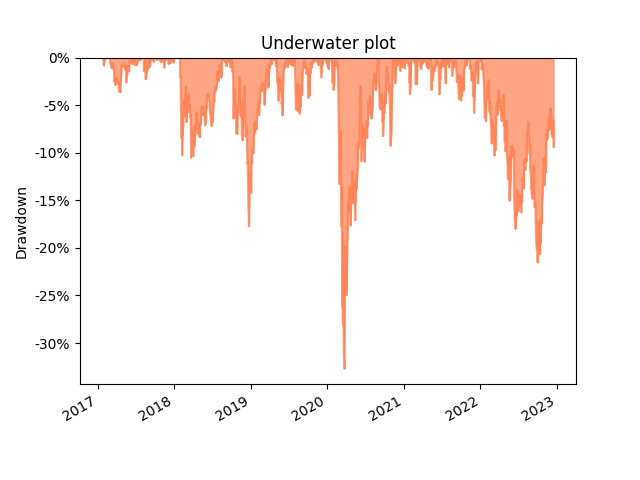
\includegraphics[width=\linewidth]{image/figure/drawdown_underwater_max}
            \caption{The model with the highest \emph{test/total\_reward}
            \label{fig:drawdown_underwater_max}}
        \end{subfigure}
        \hfill
        \begin{subfigure}[t]{\experimentimgwidth\textwidth}
            \centering
            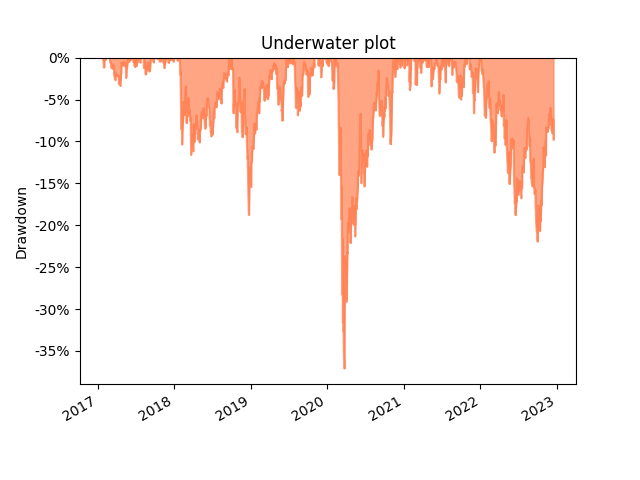
\includegraphics[width=\linewidth]{image/figure/drawdown_underwater_dji}
            \caption{The Dow Jones Industrial Average (DJI)}
            \label{fig:drawdown_underwater_dji}
        \end{subfigure}

        %
        \vspace{0.5cm}

        %
        \begin{subfigure}[t]{\experimentimgwidth\textwidth}
            \centering
            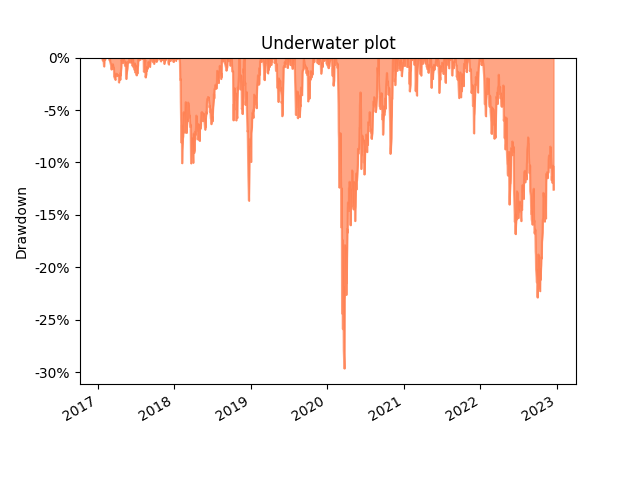
\includegraphics[width=\linewidth]{image/figure/drawdown_underwater_min}
            \caption{The model with the lowest \emph{test/total\_reward}
            \label{fig:drawdown_underwater_min}}
        \end{subfigure}
        \hfill
        \begin{subfigure}[t]{\experimentimgwidth\textwidth}
            \centering
            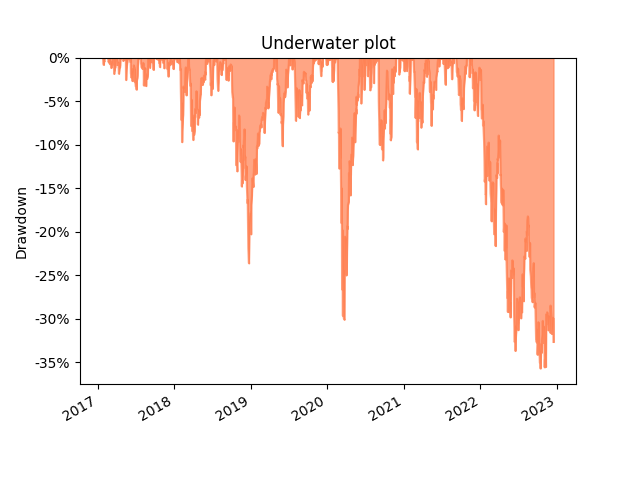
\includegraphics[width=\linewidth]{image/figure/drawdown_underwater_ixic}
            \caption{The Nasdaq 100 Index (IXIC)}
            \label{fig:drawdown_underwater_ixic}
        \end{subfigure}

        %
        \caption{Drawdown analysis of the best and worst performing models, and indexes (DJI and IXIC).}
        \label{fig:drawdown}
    \end{figure}

    \subsection{Performance of Different Portfolios: Monthly and Annualy}\label{subsec:monthly-and-annual-returns}
    In~\crefrange{fig:month_annual_returns_max}{fig:month_annual_returns_ixic}, we compared our models against baseline indexes and strategies based on their \emph{monthly} and \emph{annual} returns.\ We presented the results in a graph, where the model with the highest return was compared to the \emph{DJI} and \emph{IXIC} indexes.\ Our model consistently outperformed the DJI index in most months and years, but was outperformed by the IXIC index in 2019, 2020, and 2021.\ However, in 2022, when the IXIC index lost more than \textbf{-30\%} of its value, our model was able to keep the majority of its value and only lost less than \textbf{-8\%}.

    It's worth noting that our models achieved significant outperformance during the big drawdown period caused by the COVID-19 pandemic.\ The our model performed better than the DJI index during February, March, and April of 2020, indicating that our model was able to learn which companies with specific features were better to hold during this period.

    Although there were some months where the DJI index performed better than our models, the performance difference was not significant.\ Overall, we concluded that our models performed well in the majority of months, as demonstrated by the \emph{annual graphs}.

    It's important to note that our model was trained on companies from the DJI index, which may have influenced the comparison with the IXIC index.\ Therefore, the comparison may not be entirely fair.\ Nonetheless, the results suggest that our model is able to learn what companies to hold during certain time periods and can outperform baseline indexes.

    \begin{figure}[H]
        \centering
        \begin{subfigure}[t]{\experimentimgwidth\textwidth}
            \centering
            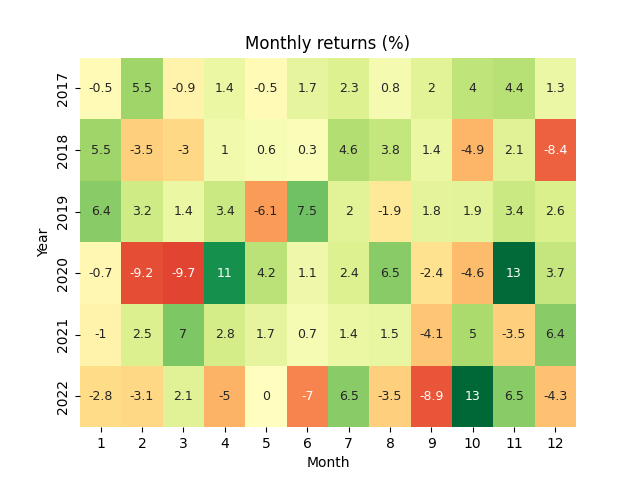
\includegraphics[width=\linewidth]{image/figure/monthly_returns_heatmap_max}
        \end{subfigure}
        \hfill
        \begin{subfigure}[t]{\experimentimgwidth\textwidth}
            \centering
            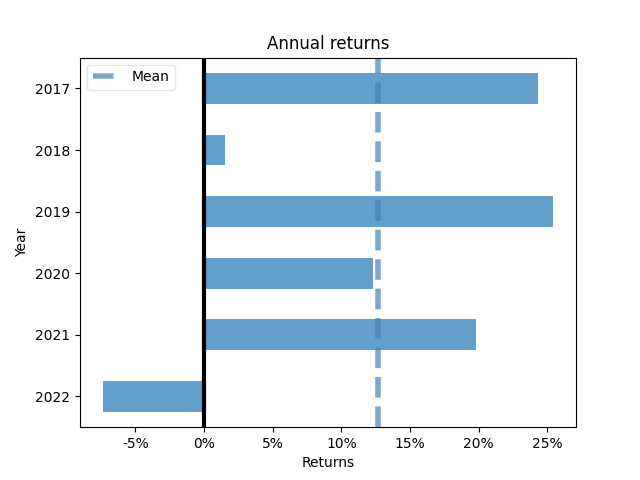
\includegraphics[width=\linewidth]{image/figure/annual_returns_max}
        \end{subfigure}
        \caption{The monthly and annual returns of the model with the highest \emph{test/total\_reward}}
        \label{fig:month_annual_returns_max}
    \end{figure}

    \begin{figure}[H]
        \centering
        \begin{subfigure}[t]{\experimentimgwidth\textwidth}
            \centering
            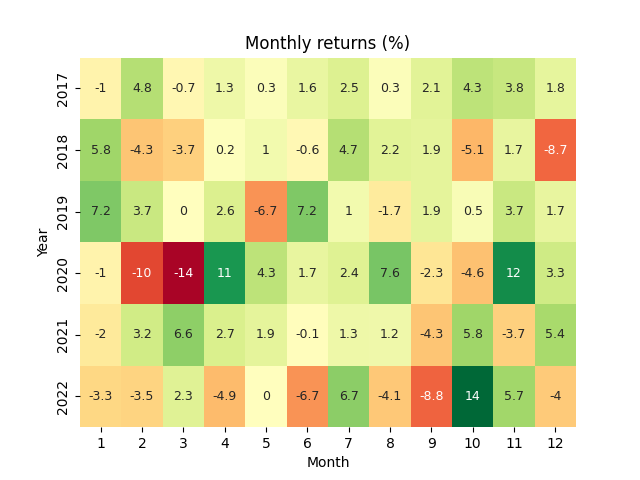
\includegraphics[width=\linewidth]{image/figure/monthly_returns_heatmap_dji}
        \end{subfigure}
        \hfill
        \begin{subfigure}[t]{\experimentimgwidth\textwidth}
            \centering
            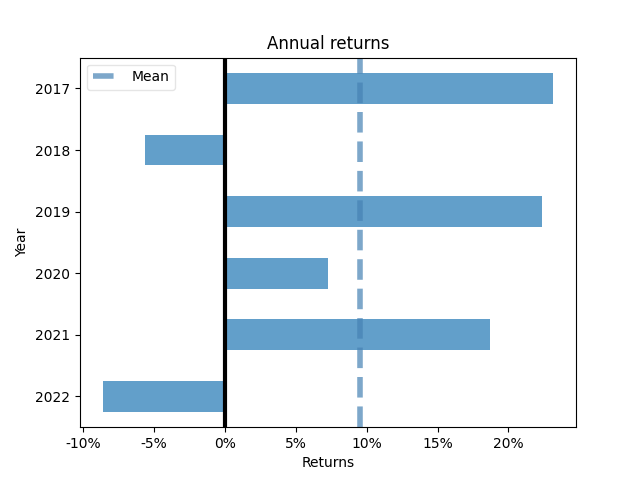
\includegraphics[width=\linewidth]{image/figure/annual_returns_dji}
        \end{subfigure}
        \caption{The monthly and annual returns of DJI Index}
        \label{fig:month_annual_returns_dji}
    \end{figure}

    \begin{figure}[H]
        \centering
        \begin{subfigure}[t]{\experimentimgwidth\textwidth}
            \centering
            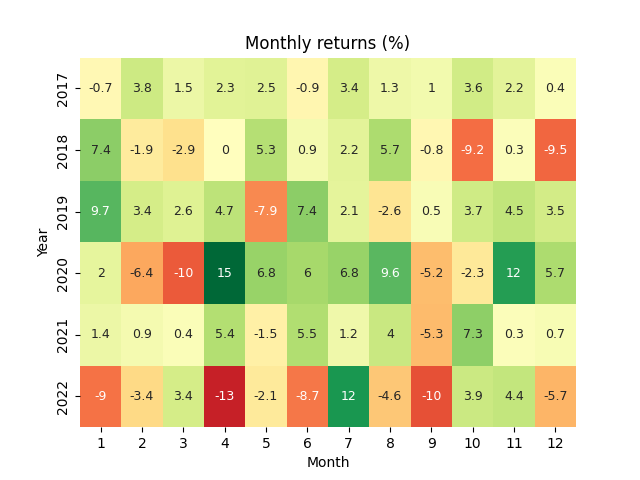
\includegraphics[width=\linewidth]{image/figure/monthly_returns_heatmap_ixic}
        \end{subfigure}
        \hfill
        \begin{subfigure}[t]{\experimentimgwidth\textwidth}
            \centering
            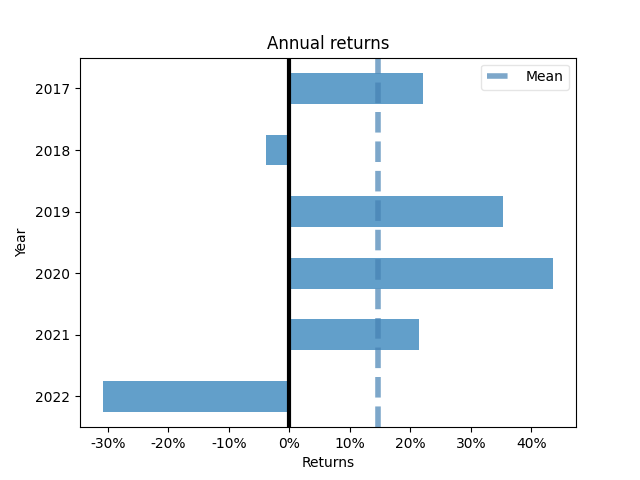
\includegraphics[width=\linewidth]{image/figure/annual_returns_ixic}
        \end{subfigure}
        \caption{The monthly and annual returns of IXIC Index}
        \label{fig:month_annual_returns_ixic}
    \end{figure}


    \section{Portfolio Metrics}\label{sec:portfolio-metrics}
    This section presents the \emph{Portfolio Metrics Comparison} of the models developed in this thesis, compared to various indexes, strategies, and a model developed by AI4Finance~\cite{finrl-portfolio-allocation-2020}.

    We do not provide an explanation of the metrics used to compare models because they are more related to Economic/Finance topics.\ However, we have referenced the Pyfolio website, where these metrics are fully described, for readers who seek additional information on the topic.\ The performance metrics were calculated using the Pyfolio framework and readers can find more information on the metrics by referring to~\cite{Pyfolio, Pyfolio-return-analysis}.

    \subsection{Comparison with State-of-the-Art AI4Finance}\label{subsec:ai4finance-model}
    The~\cref{tab:stats2} compares our models with the model from AI4Finance~\cite{finrl-portfolio-allocation-2020}.\ Due to the lack of data, we used the results from the published paper and comparison was made only for the period from \textbf{2020-07-01} to \textbf{2021-10-29}.

    As shown in the~\cref{tab:stats2}, our models are not the best compared to the AI4Finance model.\ The AI4Finance model outperforms our models in almost all performance metrics, but our models are still better than the indexes and common strategies.\ Our models were outperformed by approximately $3.1\%$ annually, which is quite significant.\ This could be due to various reasons, such as using different hyperparameters or training the models on different datasets.\ Our models were trained on a combined dataset of technical and fundamental analysis, while the AI4Finance model was trained only on technical analysis but included the covariance matrix between stocks, which we did not consider in our datasets.\ Of course it would be interesting to compare our models with the AI4Finance model over a longer period, but unfortunately, we do not have the data for that.


    \begin{table}[H]
        \centering
        {\footnotesize
            \begin{tabular}{*{4}{|m{0.20\linewidth}|}}
                \toprule
                \bfseries Metric / Model ID   & \bfseries zfjr0ks0                   & \bfseries p3irnh80                    & \bfseries AI4Finance \\[0.2cm]
                \midrule
                \bfseries Annual return       & 0.213                                & 0.265                                 & \color[HTML]{00F000} \bfseries 0.296 \\[0.2cm]
                \bfseries Cum.\ returns       & 0.295                                & 0.369                                 & \color[HTML]{00F000} \bfseries 0.415 \\[0.2cm]
                \bfseries Annual volatility   & 0.128                                & 0.130                                 & \color[HTML]{00F000} \bfseries 0.140 \\[0.2cm]
                \bfseries Sharpe ratio        & 1.573                                & 1.866                                 & \color[HTML]{00F000} \bfseries 1.930 \\[0.2cm]
                \bfseries Calmar ratio        & 2.323                                & 2.911                                 & \color[HTML]{00F000} \bfseries 3.350 \\[0.2cm]
                \bfseries Stability           & 0.893                                & \color[HTML]{00F000} \bfseries 0.931  & 0.920 \\[0.2cm]
                \bfseries Max drawdown        & -0.092                               & -0.091                                & \color[HTML]{00F000} \bfseries -0.088 \\[0.2cm]
                \bfseries Omega ratio         & 1.299                                & 1.367                                 & \color[HTML]{00F000} \bfseries 1.380 \\[0.2cm]
                \bfseries Sortino ratio       & 2.349                                & 2.792                                 & \color[HTML]{00F000} \bfseries 2.940 \\[0.2cm]
                \bfseries Skew                & -0.127                               & -0.228                                & \color[HTML]{00F000} \bfseries -0.110 \\[0.2cm]
                \bfseries Kurtosis            & 1.574                                & \color[HTML]{00F000} \bfseries 1.580  & 1.450 \\[0.2cm]
                \bfseries Tail ratio          & \color[HTML]{00F000} \bfseries 1.110 & 1.028                                 & 1.100 \\[0.2cm]
                \bfseries Daily value at risk & -0.015                               & \color[HTML]{00F000} \bfseries -0.014 & -0.017 \\[0.2cm]
                \bfseries Beta                & 0.888                                & 0.920                                 & \color[HTML]{00F000} \bfseries 0.980 \\[0.2cm]
                \bfseries Alpha               & -0.025                               & 0.009                                 & \color[HTML]{00F000} \bfseries 0.020 \\[0.2cm]
                \bottomrule
            \end{tabular}
        }
        \caption{Performance metrics of the models vs. AI4Finance model, during the testing period of 2020-07-01 to 2021-10-29.}
        \label{tab:stats2}
    \end{table}

    \subsection{Comparison with Indexes and Strategies}\label{subsec:indexes-and-strategies}
    The~\cref{tab:stats} shows the comparison of our models with the S\&P 500 (GSPC), NASDAQ Composite (IXIC), Dow Jones Industrial Average (DJI), Russell 2000 (RUT), Maximum Sharpe Ratio strategy, and Minimum Variance strategy.\ The comparison is based on the testing period from \textbf{2017-01-25} to \textbf{2022-12-16}.

    As seen in~\cref{tab:stats}, our models outperform most of the other models/strategies in almost all performance metrics.\ The \textcolor[HTML]{00F000}{\textbf{green bold values}} indicate the best results for each metric.\ However, the best values for a portfolio can vary depending on the desired outcome and other factors.

    \begin{table}[H]
        \centering
        {\footnotesize\begin{tabular}{*{9}{|m{0.075\linewidth}|}}
                          \toprule
                          \bfseries Metric / Portfolio maintainer & \bfseries zfjr0ks0 (model) & \bfseries p3irnh80 (model)           & \bfseries DJI Index                   & \bfseries GSPC Index & \bfseries IXIC Index & \bfseries RUT Index & \bfseries Max Sharpe Ratio Portfolio & \bfseries Min Variance Portfolio \\[0.4cm]
                          \midrule
                          \bfseries Annual return                 & 0.085                      & \color[HTML]{00F000} \bfseries 0.122 & 0.089                                 & 0.094                & 0.116 & 0.043 & 0.093 & 0.092 \\[0.4cm]
                          \bfseries Cum.\ returns                 & 0.621                      & \color[HTML]{00F000} \bfseries 0.972 & 0.654                                 & 0.695                & 0.911 & 0.284 & 0.686 & 0.683 \\[0.4cm]
                          \bfseries Annual volatility             & 0.181                      & 0.188                                & 0.202                                 & 0.203                & 0.239                & \color[HTML]{00F000} \bfseries 0.253 & 0.158 & 0.159 \\[0.4cm]
                          \bfseries Sharpe ratio                  & 0.543                      & \color[HTML]{00F000} \bfseries 0.706 & 0.525                                 & 0.544                & 0.581 & 0.295 & 0.641 & 0.640 \\[0.4cm]
                          \bfseries Calmar ratio                  & 0.288                      & \color[HTML]{00F000} \bfseries 0.391 & 0.241                                 & 0.276                & 0.325 & 0.101 & 0.350 & 0.349 \\[0.4cm]
                          \bfseries Stability                     & 0.855                      & \color[HTML]{00F000} \bfseries 0.913 & 0.798                                 & 0.845                & 0.820 & 0.461 & 0.905 & 0.906 \\[0.4cm]
                          \bfseries Max drawdown                  & -0.297                     & -0.312                               & -0.371                                & -0.339               & -0.357               & -0.431                               & -0.265                               & \color[HTML]{00F000} \bfseries -0.264 \\[0.4cm]
                          \bfseries Omega ratio                   & 1.118                      & \color[HTML]{00F000} \bfseries 1.158 & 1.114                                 & 1.115                & 1.116 & 1.057 & 1.136 & 1.135 \\[0.4cm]
                          \bfseries Sortino ratio                 & 0.763                      & \color[HTML]{00F000} \bfseries 0.994 & 0.723                                 & 0.751                & 0.802 & 0.404 & 0.907 & 0.904 \\[0.4cm]
                          \bfseries Skew                          & -0.249                     & -0.312                               & -0.593                                & -0.549               & -0.465               & -0.782                               & -0.246                               & \color[HTML]{00F000} \bfseries -0.240 \\[0.4cm]
                          \bfseries Kurtosis                      & 16.819                     & 19.569                               & \color[HTML]{00F000} \bfseries 19.640 & 14.205               & 7.418 & 10.450 & 14.315 & 14.286 \\[0.4cm]
                          \bfseries Tail ratio                    & 0.883                      & 0.884                                & 0.891                                 & 0.859                & 0.862                & \color[HTML]{00F000} \bfseries 0.984 & 0.937 & 0.930 \\[0.4cm]
                          \bfseries Daily value at risk           & -0.022                     & -0.023                               & -0.025                                & -0.024               & -0.030               & -0.032                               & -0.019                               & \color[HTML]{00F000} \bfseries -0.018 \\[0.4cm]
                          \bfseries Beta                          & 0.879                      & 0.921                                & 1.000                                 & 0.966                & 1.007                & \color[HTML]{00F000} \bfseries 1.083 & 0.636 & 0.637 \\[0.4cm]
                          \bfseries Alpha                         & 0.005                      & \color[HTML]{00F000} \bfseries 0.036 & 0.000                                 & 0.008                & 0.032                & -0.039 & 0.034 & 0.035 \\[0.4cm]
                          \bottomrule
        \end{tabular}}
        \caption{Performance metrics of the models vs. indexes and strategies, during the testing period of 2017-01-25 to 2022-12-15.}
        \label{tab:stats}
    \end{table}


    \section{Summary}\label{sec:summary}
    In this chapter, we conducted empirical experiments to evaluate how well a Deep Reinforcement Learning (DRL) agent can perform in the portfolio management task.\ Our results show that DRL has a huge potential in portfolio allocation as it can outperform common strategies and indexes.\ We used DRL algorithms to explore the relationship between the reward (i.e., portfolio return) and the input (i.e., features) and measured the prediction power using portfolio metrics.\ We found that the Fundamental Features or a combination of Fundamental and Technical Analysis features can effectively describe the environment and be used to train DRL agents.

    Portfolio management is a challenging task that requires a lot of data, which is often expensive and difficult to obtain.\ Our Stock Portfolio Allocation Environment, modeled using MDP, aims to identify how stocks are valued and which State Space features affect price movements.\ We assume that the Financial Market operates like any other market where the price of a stock or asset increases when people buy it and decreases when people sell it.\ Therefore, our model attempts to predict how much each feature affects future price movements (people's interest to buy/sell).\ Since the Stock Market is predominantly controlled by ``Big Money'' players such as banks and hedge funds, we believe that our research is crucial for portfolio managers to improve their decision-making capabilities.

    In addition to the future work mentioned earlier, we see a great opportunity to extend our model by incorporating a system that automatically places orders to the broker based on the weight predicted by our model.\ This would streamline the entire process of portfolio management and eliminate the need for manual intervention.

    Furthermore, we believe that our model can benefit from the inclusion of additional features such as sentiment analysis, macroeconomic factors, and industry-specific factors.\ The inclusion of these features can help our model to better capture the market's behavior and improve its performance.

    Another area of improvement that we believe warrants further exploration is the reward function.\ While our experiments have shown that the reward function we used was effective to some extent, we acknowledge that it may not capture all the nuances of the market.\ Therefore, we recommend exploring alternative reward functions that can better account for the goodness or badness of actions taken by the agent.

    Overall, we believe that our study has demonstrated the potential of DRL in portfolio allocation, but there are still many avenues for improvement and further research.\ By incorporating these future works, we can enhance the performance of our model and make it more suitable for real-world applications.
\end{document}
